\documentclass[11pt]{article}
\usepackage[margin = 1in]{geometry}
\usepackage{amsmath}
\usepackage{amssymb}
\usepackage{amsthm}
\usepackage{graphicx}
\usepackage{enumitem}
\usepackage{url}
\usepackage[parfill]{parskip}
\usepackage{listings}
\newcommand{\skipline}{\vspace{\baselineskip}}
\newcommand{\spacer}{\noalign{\medskip}}
\newenvironment{problem}[1]{\textbf{Problem #1: }}{\newpage}
\usepackage{caption}
\usepackage{subcaption}
\usepackage[utf8]{inputenc}
\usepackage{xcolor}
\definecolor{codegreen}{rgb}{0,0.6,0}
\definecolor{codegray}{rgb}{0.5,0.5,0.5}
\definecolor{codepurple}{rgb}{0.58,0,0.82}
\definecolor{backcolour}{rgb}{0.95,0.95,0.92}
\lstdefinestyle{mystyle}{
	backgroundcolor=\color{backcolour},   
	commentstyle=\color{codegreen},
	keywordstyle=\color{magenta},
	numberstyle=\tiny\color{codegray},
	stringstyle=\color{codepurple},
	basicstyle=\ttfamily\footnotesize,
	breakatwhitespace=false,         
	breaklines=true,                 
	captionpos=b,                    
	keepspaces=true,                 
	numbers=left,                    
	numbersep=5pt,                  
	showspaces=false,                
	showstringspaces=false,
	showtabs=false,                  
	tabsize=2
}
\lstset{style=mystyle}
\newcommand{~}{\sim}

\begin{document}
	
	\begin{center}
		\textbf{Homework 6} \\
		\textbf{Ordinary Differential Equations} \\
		\textbf{Math 537} \\
		\textbf{Stephen Giang RedID: 823184070} \\
		\skipline \skipline
	\end{center}

	\begin{problem}{1}
		Compute the Picard iterations for the initial value problem:
		\[\frac{dy}{dt} = ay, \qquad y(t = 0) = 1.\]
		Notice the following:
		\\ \\
		Let $u_0(t) = 1, F(y) = ay$
		\begin{align*}
			u_0(t) &= 1 \\
			u_1(t) &= 1 + \int_{0}^{t} F(u_0(s))\,ds = 1 + a\int_{0}^{t} ds = 1 + at \\
			u_2(t) &= 1 + \int_{0}^t F(u_1(s))\,ds = 1 + a\int_{0}^t (1 + as)\,ds = 1 + at + \frac{a^2t^2}{2} \\
			u_3(t) &= 1 + \int_{0}^t F(u_2(s))\,ds = 1 + a\int_{0}^t \left(1 + as + \frac{a^2s^2}{2}\right)\,ds \\
			&= 1 + at + \frac{(at)^2}{2} + \frac{(at)^3}{6} \\
			u_k(t) &= \sum_{n = 0}^{k} \frac{(at)^n}{n!}
		\end{align*}
		\[\boldsymbol{\textbf{As }k \rightarrow \infty, u_k(t) = \sum_{n = 0}^{k} \frac{(at)^n}{n!} = e^{at}}\]
	\end{problem}

	\begin{problem}{2}
		 Consider the following second-order homogeneous nonlinear differential equation:
		 \[\frac{d^2X}{dt^2} + h\left(X, \frac{dX}{dt}\right) + g\left(X\right) = 0.\]
		 Let 
		 \[E = \frac{1}{2}\left(\frac{dX}{dt}\right)^2 + \int g\left(X\right)dX.\]
		 \begin{enumerate}[label = (\alph*)]
		 	\item Show that $\frac{dE}{dt} = -h\frac{dX}{dt}$.
		 	\\ \\
		 	Notice the following:
		 	\begin{align*}
		 		\frac{dE}{dt} &= \frac{dX}{dt}\frac{d^2X}{dt^2} + \frac{dX}{dt}\frac{d}{dx}\int g(X) \\
		 		&= \left(\frac{d^2X}{dt^2} + g(X)\right)\frac{dX}{dt} \\
		 		&= -h\frac{dX}{dt}
		 	\end{align*}
		 	\item Consider the Van der Pol equation:
		 	\[\frac{d^2X}{dt^2} + \mu \left(X^2 - 1\right)\frac{dX}{dt} + X = 0.\]
		 	Discuss the conditions under which $\frac{dE}{dt}$ is positive (and negative)
		 	\\ \\
		 	Notice the following:
		 	\[h(X, \frac{dX}{dt}) = \mu \left(X^2 - 1\right)\frac{dX}{dt} \qquad \frac{dE}{dt} = -h\frac{dX}{dt} = -\mu \left(X^2 - 1\right)\left(\frac{dX}{dt}\right)^2\]
		 	Notice the following:
		 	\[\left(\frac{dX}{dt}\right)^2 \geq 0\]
		 	\textbf{\boldmath Let $\mu > 0$, we get the following results:}
			\begin{enumerate}[label = (\alph*)]
				\item For $\frac{dE}{dt} < 0$ (negative),  $X^2 - 1 > 0$, such that $|X| > 1$. \\
				\item For $\frac{dE}{dt} > 0$ (positive),  $X^2 - 1 < 0$, such that $|X| < 1$.
			\end{enumerate}
			\skipline
		 	\textbf{\boldmath For $\mu < 0$, we get the following results:}
		 	\begin{enumerate}[label = (\alph*)]
		 		\item For $\frac{dE}{dt} < 0$ (negative),  $X^2 - 1 < 0$, such that $|X| < 1$. \\
		 		\item For $\frac{dE}{dt} > 0$ (positive),  $X^2 - 1 > 0$, such that $|X| > 1$.
		 	\end{enumerate}
		 \end{enumerate}
	\end{problem}

	\begin{problem}{3}
		Consider the following second-order differential equation
		\[x\frac{d^2y}{dx^2} + \frac{dy}{dx} = y,\]
		which has an irregular singular point at $\infty$. Apply the substitution $y = e^{S(x)}$
		to show that the leading behavior of $y(x)$ is given by
		\[y(x) \sim cx^{-1/4}e^{2x^{1/2}}, x \rightarrow +\infty\]
		here $c$ is a constant.
		\\ \\
		Notice the following:
		\[y = e^{S(x)} \qquad \frac{dy}{dx} = S'(x)e^{S(x)} \qquad \frac{d^2y}{dx^2} = \left( S''(x) + (S'(x))^2\right) e^{S(x)}\]
		We can rewrite it as follows:
		\begin{align*}
			x\left( S'' + (S')^2\right) e^{S(x)} + S'e^{S(x)} - e^{S(x)} &= 0 \\
			xS'' + x(S')^2 + S' - 1 &= 0 
		\end{align*}
		Now we can drop the all the small terms and rewrite the equation:
		\[x(S')^2+S'-1 \sim 0, \qquad x \rightarrow \infty, \tag{1}\]
		Now we can see the following:
		\[S' \sim \frac{-1 \pm \sqrt{1 + 4x}}{2x} \sim \pm \frac{1}{\sqrt{x}}, \qquad x \rightarrow \infty\]
		Thus we get:
		\[S(x) = 2\sqrt{x} + C(x)\]
		with $C(x) << 2\sqrt{x}, C' << x^{-1/2}, C'' << x^{-3/2}$.
		\\ \\
		If we substitute this into equation (1) and combine the $C(x)$ terms, we get:
		\[xC'' + x(C')^2 + (2\sqrt{x} + 1 )C' + \frac{1}{2\sqrt{x}} = 0\]
		Notice the following from the facts about $C(x)$:
		\[1 << 2\sqrt{x}, \qquad xC'' << \frac{1}{2\sqrt{x}}, \qquad x(C')^2 << 2\sqrt{x}C', \qquad x \rightarrow \infty\]
		Thus we get 
		\[2\sqrt{x}C' \sim -\frac{1}{2\sqrt{x}}, \qquad C' ~ -\frac{1}{4x}\]
		Thus we get that 
		\[C(x) = \frac{-1}{4}\ln x + d\]
		Finally, this leads to the following:
		\[S(x) = 2\sqrt{x} + \frac{-1}{4}\ln x + d\]
		Notice that this shows the leading behavior:
		\[\boldsymbol{y ~ e^{S(x)} ~ e^{2x^{1/2}}e^{-(1/4)\ln x}e^d ~ cx^{-1/4}e^{2x^{1/2}}, \qquad x \rightarrow \infty}\]
	\end{problem}

	\begin{problem}{4}
		 Consider a boundary-layer problem with the following second order linear differential equation:
		 \[\epsilon\frac{d^2y}{dx^2} + (1 + \epsilon)\frac{dy}{dx} + y = 0,\]
		 \[y(0) = 0 \text{ and } y(1) = 1.\]
		 \begin{enumerate}[label = (\alph*)]
		 	\item Solve for the exact solution.
		 	\\ \\
		 	Notice we can get the characteristic equation:
		 	\[\epsilon \lambda^2 + (1 + \epsilon)\lambda + 1 = 0\]
		 	Now notice the lambda values from the quadratic equation:
		 	\begin{align*}
		 		\lambda &= \frac{1}{2\epsilon}\left(-(1 + \epsilon) \pm \sqrt{(1 + \epsilon)^2 - 4\epsilon} \right) \\
		 		&= \frac{1}{2\epsilon}\left(-(1 + \epsilon) \pm \sqrt{\epsilon^2 + 2\epsilon + 1 - 4\epsilon} \right) \\
		 		&= \frac{1}{2\epsilon}\left(-(1 + \epsilon) \pm \sqrt{\epsilon^2 - 2\epsilon + 1} \right) \\
		 		&= \frac{1}{2\epsilon}\left(-(1 + \epsilon) \pm \sqrt{(\epsilon - 1)^2} \right) \\
		 		&= \frac{1}{2\epsilon}\left(-(1 + \epsilon) \pm (\epsilon - 1) \right) \\
		 		&= \frac{-1}{\epsilon}, \quad -1
		 	\end{align*}
	 		So we get the following general solution:
	 		\[y = c_1e^{-x} + c_2e^{-x/\epsilon}\]
	 		Notice the matrix and its reduced row echelon form found through the Maple Software:
	 		\[\left[\begin{array}{ccc}
	 			1&1&0 \\
	 			\spacer e^{-1} & e^{-1/\epsilon} & 1
	 		\end{array}\right] \qquad \xrightarrow{rref} \qquad \left[\begin{array}{ccc}
	 			1&0&\frac{-1}{e^{-1/\epsilon} - e^{-1}} \\
	 			\spacer 0&1&\frac{1}{e^{-1/\epsilon} - e^{-1}} \\
 			\end{array}\right]\]
	 		Thus we get the following exact solution:
	 		\[\boldsymbol{y = \frac{e^{-x/\epsilon} - e^{-x}}{e^{-1/\epsilon} - e^{-1}}}\]
	 		\newpage
		 	\item Plot the solution for $\epsilon = 0.01, 0.05,$ and $0.1$. 
		 	\begin{figure}[h!]
		 		\centering
		 		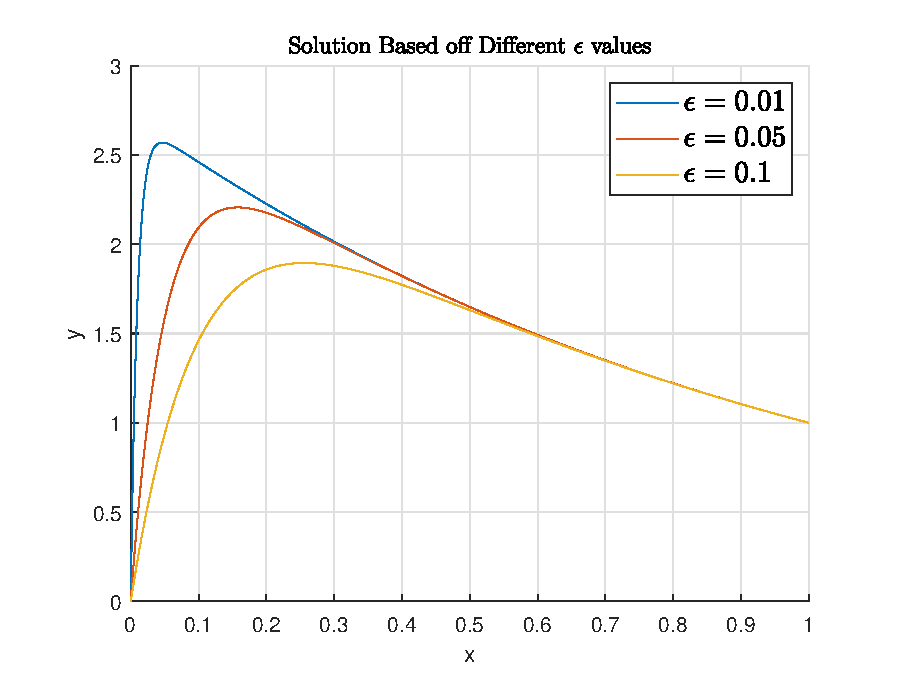
\includegraphics[width = .7\textwidth]{Prob4b}
		 	\end{figure}
		 	\item Determine the inner and outer limit of the solution.
		 	\\ \\
		 	Notice the following for the outer limit:
		 	\[\boldsymbol{ \lim\limits_{\epsilon \rightarrow 0} y(x) = \frac{e^{-x}}{e^{-1}} = e^{1 - x} }\]
		 	Let $x = \epsilon\mathbb{X}$ and notice the following for the inner limit:
		 	\[\boldsymbol{ y = \frac{e^{-\mathbb{X}} - e^{-\epsilon\mathbb{X}}}{e^{-1/\epsilon} - e^{-1}} \qquad \lim\limits_{\epsilon \rightarrow 0} y(x) = \frac{e^{-\mathbb{X}} - 1}{-e^{-1}} = e - e^{1 - \mathbb{X}} }\]
		 	Thus we get the following: 
		 	\[\boldsymbol{ \mathbb{Y} \sim  e^{1 - x} - e^{1 - \mathbb{X}} }\]
		 \end{enumerate}
	\end{problem}
\end{document}
